\documentclass[english,11pt]{article}
\usepackage[table]{xcolor}
\usepackage{color}
\usepackage{amsmath}
\usepackage{amsmath}
\usepackage{amssymb}
\usepackage{color}
\usepackage{tikz,graphicx}
\usetikzlibrary{positioning,arrows.meta,calc,decorations.pathreplacing}

\begin{document}

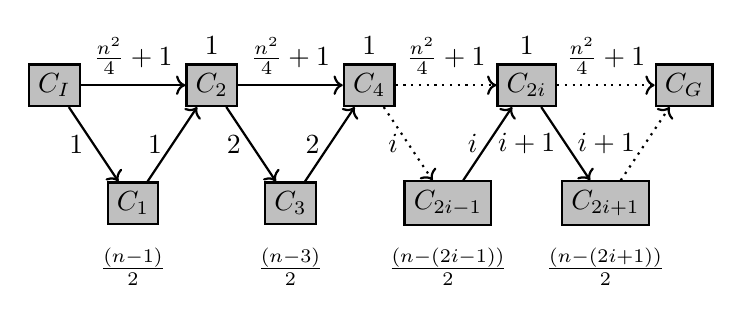
\begin{tikzpicture}[thick,scale=1]
     % Villes
  \node[draw, fill=black!25] (0) at (-2,0) {$C_I$};
  \node (1.l) at (0,0.5) {1};
  \node[draw, fill=black!25] (1) at (0,0) {$C_2$};
  \node (2.l) at (-1,-2.3) {$\frac{(n-1)}{2}$};
  \node[draw, fill=black!25] (2) at (-1,-1.5) {$C_1$};
  \node (3.l) at (2,0.5) {1};
  \node[draw, fill=black!25] (3) at (2,0) {$C_4$};
  \node (4.l) at (1,-2.3) {$\frac{(n-3)}{2}$};
  \node[draw, fill=black!25] (4) at (1,-1.5) {$C_3$};
  \node (5.l) at (4,0.5) {1};
  \node[draw, fill=black!25] (5) at (4,0) {$C_{2i}$};
  \node (6.l) at (3,-2.3) {$\frac{(n-(2i-1))}{2}$};
  \node[draw, fill=black!25] (6) at (3,-1.5) {$C_{2i-1}$};
  \node[draw, fill=black!25] (7) at (6,0) {$C_G$};
  \node (8.l) at (5,-2.3) {$\frac{(n-(2i+1))}{2}$};
  \node[draw, fill=black!25] (8) at (5,-1.5) {$C_{2i+1}$};
 
     % Liaison inter villes
  \draw[thick, ->] (0) -- node[midway, above]{$\frac{n^2}{4}+1$} (1);
  \draw[thick, ->] (0) -- node[left]{1} (2);
  \draw[thick, ->] (2) -- node[left]{1} (1);

  \draw[thick, ->] (1) -- node[midway, above]{$\frac{n^2}{4}+1$}(3);
  \draw[thick, ->] (1) --node[left]{2} (4);
  \draw[thick, ->] (4) --node[left]{2} (3);

  \draw[dotted, ->] (3) -- node[midway, above]{$\frac{n^2}{4}+1$} (5);
  \draw[dotted, ->] (3) --node[left]{$i$} (6);
  \draw[thick, ->] (6) --node[left]{$i$} (5);
  
  \draw[dotted, ->] (5) -- node[midway, above]{$\frac{n^2}{4}+1$} (7);
  \draw[thick, ->] (5) --node[left]{$i+1$} (8);
  \draw[dotted, ->] (8) --node[left]{$i+1$} (7);

\end{tikzpicture}

\end{document}